\documentclass[10pt,twocolumn]{article}

\usepackage[margin=30pt]{geometry}
\usepackage{amsmath}
\usepackage{physics}
\usepackage{amssymb}
\usepackage{amsfonts}
\usepackage{hyperref}
\usepackage{thmbox}
\usepackage{geometry}
\usepackage{graphicx}
\usepackage[]{subcaption}

\newcommand{\R}{\mathbb{R}}
\newcommand{\C}{\mathbb{C}}

\renewcommand{\thefootnote}{\fnsymbol{footnote}}

\author{Haiyang Wang, Nils Jan Fredrik Fryklund, Samuel Potter, Leslie Greengard}
\date{\today}
\title{A Fast Solver for Stokes Flow in 2D: [we need a better title]}

\begin{document}

\maketitle

\begin{abstract}
  In this paper, we exploit the \textit{return to Poiseuille} phenomenon: 
  a Stokes flow would quickly develop to the Poiseuille flow along a straight channel. 
  This allows us to quickly solve the interior plane Stokes equation 
  on a domain that is a union of \textit{standard pieces}. 
  Each standard piece is a pipe with inlets/outlets 
  being long enough straight channels, such that when two standard pieces are connecting,
  where they connect is in middle of a long
  straight channel\footnote{
  The length of straight channel is greater than 7 times of the width, 
  as indicated by Figure \ref{fig:r2pnumerical}}, hence the flow 
  at the connection would be close to Poiseuille flow up within machine precision. 
  Therefore, instead of solving stokes equation for the global domain, 
  we can solve the Stokes equation 
  for each standard pieces with Poiseuille 
  boundary condition at inlets/outlets, 
  and easily interface these local solutions 
  to build a solution for the global domain. 
  
  Once the Stokes equation with Poiseuille boundary conditions is pre-solved on each standard piece, 
  the standard pieces can be connected to form a complex domain of channel network. 
  Interfacing the solutions of standard pieces
  would instantly give a high-order accurate solution of Stokes equation 
  for the global domain. 
  For example, in Figure \ref{fig:connection-error}, interfacing the local solutions took only 0.3 seconds, while directly
  solving on the global domain took 24 minutes. 
\end{abstract}

\begin{figure*}[t] 
  \centering
  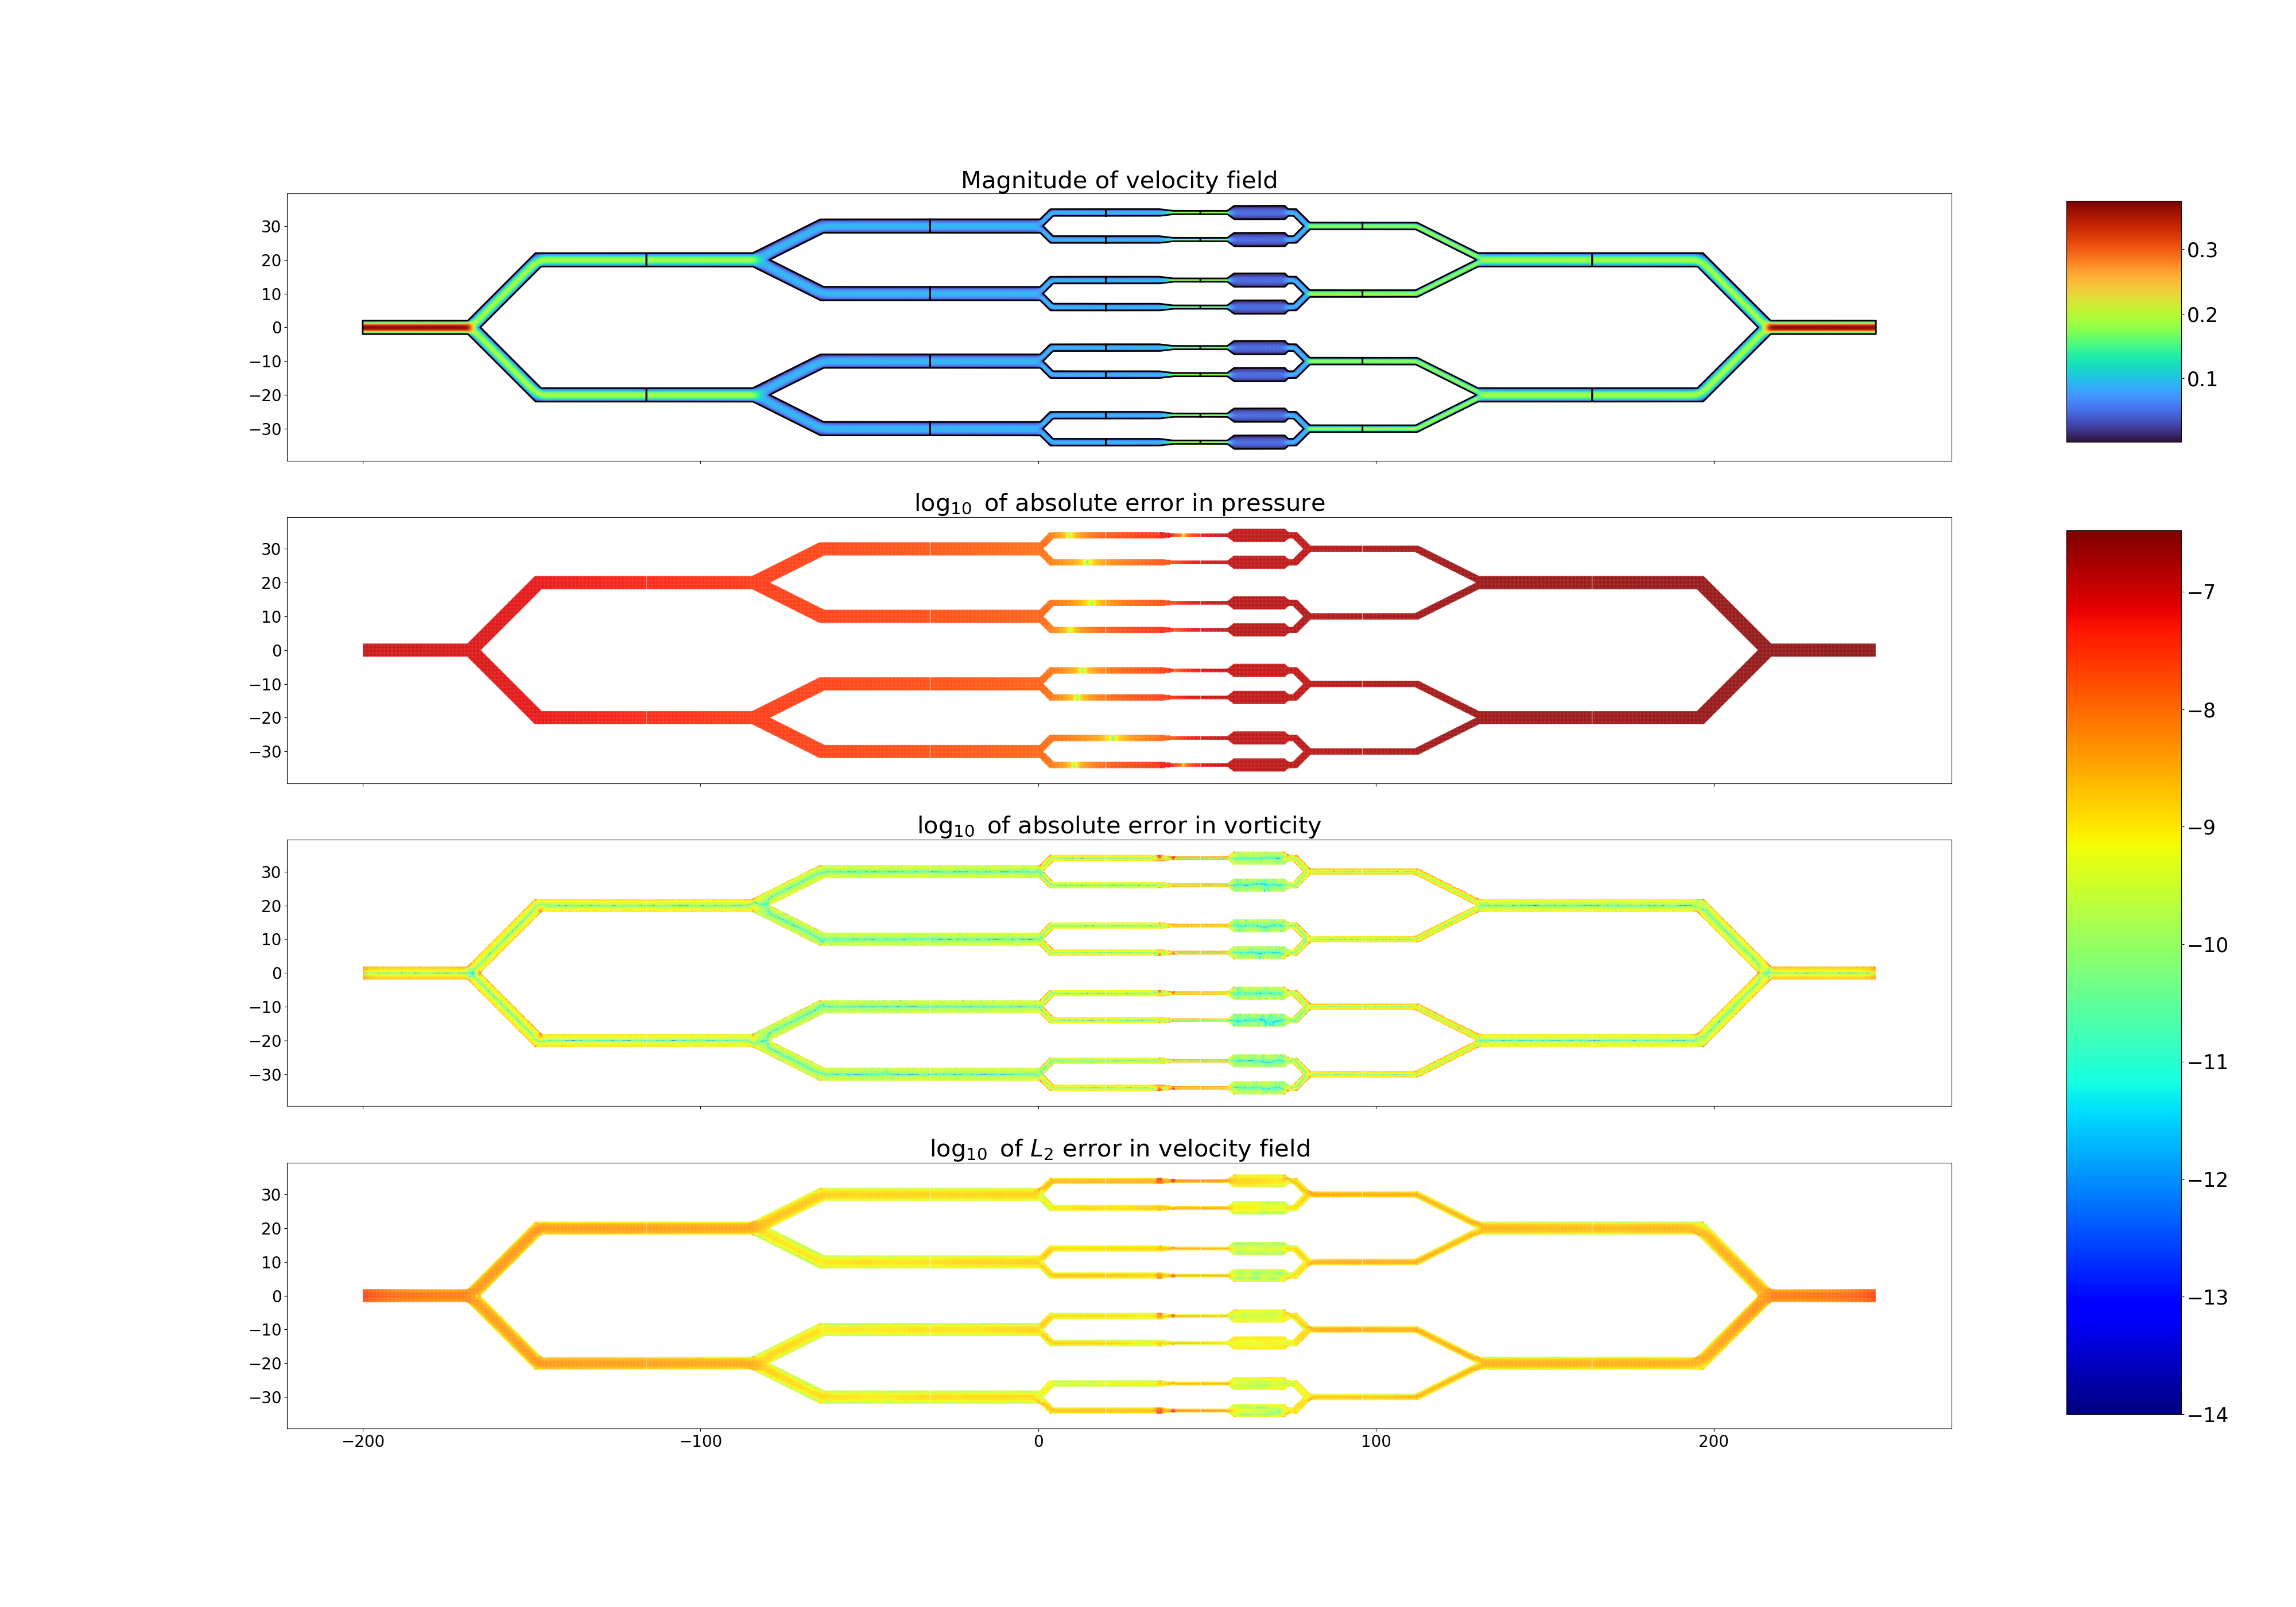
\includegraphics[width=\textwidth]{pic/connection-error-rough.png}
  \caption{Solutions of the Stokes equation in a complex channel geometry as a union of 22 standard pieces
    with Poiseuille velocity profile of unit flux given at the left inlet and right outlet, and non-slippery boundary conditions elsewhere, 
    The first sub-figure is a color-plot of magnitude of velocity field inside the 
    domain, with colorbar on its right. The black lines in the 
    first sub-figure marks the boundary of each standard piece. 
    The other three sub-figures is color plot of absolute differences 
    between the connected solution and the global solution in pressure, 
    vorticity, and velocity field in the $log_{10}$ scale. Each standard pieces are solved
    with required accuracy of $10^{-12}$ and the global domain is solved with 
    required accuracy of $10^{-10}$.}
  \label{fig:connection-error}

\end{figure*}

\section{Introduction}


The \textit{return to Poiseuille} phenomenon, or \textit{Saint-Venant's principle} in the theory of plane elasticity, 
are well-established from the last century 
\cite{coRecentDevelopmentsConcerning1983,gregoryTractionBoundaryValue1980,horganDECAYESTIMATESBIHARMONIC1989}. 
To be more specific, in a straight channel with laminar and incompressible incoming flow, the differences of Stokes flow and Poiseuille flow would decay exponentially fast toward the outlet. 
Therefore it is a good numerical hypothesis to assume that the flow is Poiseuille in middle of a lone straight channel.

For plane Stokes flow, the biharmonic equation formulation are well known 
and developed within theory of complex variable from the last century \cite{ladyzhenskayaMathematicalTheoryViscous1964}. 
Various numerical schemes, such as boundary integral equation (BIE) and rational function approximation, 
have been developed accordingly \cite{greengardIntegralEquationMethods1996,trefethenApproximationTheoryApproximation2019}. 

In this paper, we use the biharmonic BIE formulation for the plane Stokes equation from 
\cite{greengardIntegralEquationMethods1996} to solve the Stokes equation on several standard pieces 
with Poiseuille boundary condition at inlets/outlets. 
The biharmonic BIE is coupled with a Fast Multiple Method (FMM) for 2D biharmonic equation
to reduce the time and space complexity of solving the BIE. \cite{FlatironinstituteFmm2d2022} 

Directly evaluating the BIE's solution near the boundary could be numerically unstable as the integral is nearly-singular.
Thus, we have adopted the methods from 
\cite{wuSolutionStokesFlow2020,helsingEvaluationLayerPotentials2008} 
for accurate evaluation of layer potentials near the boundary. 

The main idea of this paper is to apply \textit{Return to Poiseuille} as a 
high order accurate numerical hypothesis. It allows us to pre-solve a few standard pieces
which have inlets and outlets that are long enough straight channels, 
with Poiseuille boundary condition at inlets/outlets. 
Once the standard pieces are pre-solved, 
the \textit{Return to Poiseuille} hypothesis allows us to interface solutions of stokes flow on 
each standard pieces to get a solution for any complex channel networks that is a disjoint union of 
the standard pieces. 
Interfacing is by solving a system of linear equations, 
based on the constraints of flux and continuity of pressure. 
This system of linear equations depends on the flux and pressure only at where the standard pieces are connected, 
and can be solved instantly and accurately. 

This paper is organized as follows. In Section \ref{mathprelim}, we define the Stokes boundary value problem, 
the corresponding biharmonic boundary value problem, and then the integral equation of it. 
We also mention the analytic evidence and predicted exponential convergence rate for the 
\textit{return to Poiseuille} hypothesis in a long straight channel. 
Then, we explain how to interfacing the local solutions of standard pieces by an simple example. 
In Section \ref{sec:numericalmethod}, we presents the Nystr\"om discretization
of the integral equation, which is solved iteratively by 
Generalized Minimal Residual Method (GMRES). 
% At the end of this section, we also points to the 
% reference of other techniques we have adopted in this paper: 
% accurate evaluation of nearly singular integral, 
% GMRES with removed nullspace, 
% the smoothing of corners of the geometry,
% and the biharmonic FMM. 
The numerical experiments of connecting standard pieces and numerical evidence for \textit{return to Poiseuille}
hypothesis are contained in Section \ref{sec:numericalresults}, 
followed by conclusions and possible further work in Section \ref{sec:conclusions}.


\section{Mathematical Preliminaries\label{mathprelim}}

In this section, we briefly review the plane Stokes equation, its biharmonic form,
and the biharmonic boundary integral equation. More detailed discussion can be found in 
\cite{greengardIntegralEquationMethods1996}. 
Then, we will present an analytic estimate for the exponential decay rate of 
\textit{return to Poiseuille} hypothesis \cite{gregoryTractionBoundaryValue1980}, 
and explain how we have applied it as a numerical hypothesis: 
how to build local solutions for each standard pieces
and how to interface the local solutions. 

\subsection{Boundary Integral Equation}

\paragraph{Stokes Boundary Value Problem.}

Recall that the plane Stokes equations are:
\begin{align}
  \nu \Delta u = \frac 1 \rho \pdv{p}{x},\quad &\nu \Delta v = \frac 1\rho \pdv{p}{y} 
  \label{stokes} \\
  \pdv{u}{x} + \pdv{v}{y} &= 0
  \label{continuity}
\end{align}
where $u,v$ are components of velocity, $p$ is the pressure, 
$\rho$ and $\nu$ are the density and viscosity, which are constants.  
Another important physics quantity, vorticity, is defined as $\zeta  = u_y - v_x$. 

We are interested in Dirichlet boundary value problem (BVP) of Stokes equation on 
a bounded $(M+1)$-ply connected domain $D\subset \mathbb R^2$,
with boundary $\partial D =  \Gamma = \Gamma_0 \cup \Gamma_1 \cup \cdots \cup \Gamma_M$, 
where $\Gamma_0$ is the exterior boundary, and $\Gamma_1,\cdots, \Gamma_M$ are the interior boundaries. 
On the boundary $\Gamma$, the velocity is defined by given functions $h_1,h_2$:
\begin{align}
  u = h_2(t),\quad v = - h_1(t), \quad t\in \Gamma
  \label{bdr-velocity}
\end{align}
For the specific purpose of this paper, 
the boundary velocity profile is zero everywhere except at the inlets/outlets
of channels, where a Poiseuille velocity profile is specified. 

\paragraph*{Biharmonic Equation.} $(\ref{continuity})$ implies the existence of the stream function $W(x,y)$ such that:
\begin{align}
  \pdv{W}{x} = -v,\quad \pdv{W}{y} = u \label{stream-1}
\end{align}

Following (\ref{stokes},\ref{continuity}), it is easy to see that the stream function satisfies the biharmonic equation (\ref{biharmonic}),
and the Dirichlet BVP ($\ref{bdr-velocity}$) can be understood as 
the following biharmonic BVP:
\begin{align}
  &\Delta^2 W(x,y) = \Delta \zeta = 0, &(x,y)\in D \label{biharmonic}\\
  &\pdv{W}{x}(t) = h_1(t),\quad \pdv{W}{y}(t) = h_2(t), \quad &t\in \Gamma\label{bih-bv}
\end{align}
% where $h_1,h_2$ are from equation (\ref{bdr-velocity}).

\paragraph*{Goursat's Formula.} It has been long established that any plane biharmonic function $W(x,y)$ can be expressed by Goursat's formula 
\begin{align}
  W(x,y) = \Re (\bar z \phi(z) + \chi (z)) \label{Goursat}
\end{align}
where the Goursat's functions $\phi, \chi$ are analytic functions of complex variable $z = x+yi$.
In the following, we will be identifying $(x,y) \in \mathbb{R}^2$ with $x + yi \in \mathbb{C}$. 

Velocity, pressure, and vorticity can be conveniently expressed with the Goursat's functions. 
The Muskhelishvili's formula \eqref{muskhelishvili} 
expresses velocity field and another formula \eqref{pressure-and-vorticity} gives the pressure and vorticity:
\begin{align}
  -v + ui &= \pdv{W}{x} + i\pdv{W}{y} 
    = \phi(z) + z \overline{\phi'(z)} + \overline{\psi(z)}
    \label{muskhelishvili}\\
   \zeta + \frac{i}{\nu}p &= 4\phi'(z) \label{pressure-and-vorticity}
\end{align} where $\psi = \chi'$ \cite{muskhelishviliBasicProblemsMathematical1977}. 

The biharmonic boundary value problem (\ref{biharmonic},\ref{bih-bv}), 
using the Muskhelishvili's formula (\ref{muskhelishvili}), can be rewritten as
\begin{align}
  \phi(t) + t\overline{\phi'(t)} + \overline{\psi(t)} 
  = h(t), \quad
  t \in \Gamma \label{musk-bvp}
\end{align} where $h(t) =  h_1(t) + ih_2(t)$,  and $t$ is understood as a complex variable. 

\paragraph*{Sherman-Lauricella Representation.} 
The Sherman-Lauricella Representation proposes a specific form of the Goursat's functions. And one can use this representation as an ansatz for BIE of the Biharmonic BVP \eqref{musk-bvp}
\cite{greengardIntegralEquationMethods1996}. 
The Sherman-Lauricella representation is formulated as follows:
\begin{align}
  \phi(z) &=
    \frac {1}{2\pi i} \int_\Gamma \frac{\omega(\xi)}{\xi - z} d\xi  
    + \sum_{k=1}^M C_k \log (z-z_k) \label{sl-phi}
    \\
  \psi(z) &=
    \frac {1}{2\pi i} \int_\Gamma \frac{\overline{\omega(\xi)}d\xi +  \omega(\xi)\overline{d\xi}}{\xi - z}  
    - \frac {1}{2\pi i} \int_\Gamma \frac{\overline{\xi} \omega(\xi)}{(\xi - z)^2} d\xi  \label{sl-psi}
    \\
    & \quad + \sum _{k=1}^M 
    \left( \frac{b_k}{z-z_k} + \overline C_k \log (z-z_k) -  C_k \frac{\overline z_k}{z-z_k} \right) \nonumber 
\end{align}
where $\omega$ is an unknown complex density on $\Gamma$ to be solved 
for with the given $h$, 
$z_k$ are arbitrarily prescribed point inside the component curves $\Gamma_k$, 
and $C_k, b_k$ are constants defined by 
\begin{align}
  C_k = \int_{\Gamma_k} \omega(\xi) |d\xi|, \quad b_k = 2 \Im\int_{\Gamma_k} \overline{\omega(\xi)} {d\xi}
\end{align}

\paragraph*{Boundary Integral Equation.} 
Plugging the Sherman-Lauricella representation (\ref{sl-phi},\ref{sl-psi}) into equation (\ref{musk-bvp}), 
and letting a point $z$ in the interior of $D$ approach to a point on the boundary $t\in \Gamma$ in \eqref{musk-bvp}, 
the classical formulae for the limiting values of Cauchy-type integral 
gives us the following integral equation for $\omega$ \cite{muschelisviliSingularIntegralEquations1972,greengardIntegralEquationMethods1996}:
\begin{align}
  \omega(t) 
  &+ \frac 1{2\pi i} \int_{\Gamma} \omega(\xi) d\ln \frac{\xi - t}{\overline{\xi - t}} - \frac 1{2\pi i} \int_\Gamma \overline{\omega(\xi)} d \frac{\xi - t}{\overline{\xi - t}} \label{bie} \\
  &+ \sum_{k=1}^M \left( \frac{\bar b_k}{\overline{t- z_k}} +  2C_k \log |t-z_k| + \overline{C_k} \frac{t-z_k}{\overline{ t - z_k}} \right) \nonumber\\
  &+ \frac{\overline b_0}{\overline{ t - z^*}} \nonumber \\
  &= h(t) \nonumber
\end{align}
the extra term $\frac{\overline b_0}{\overline{t - z^*}}$ vanishes when the zero-net-flux condition $\Re \int_\Gamma \bar h(t) dt = 0$ is satisfied, hence will be omitted in the Nystr\"om discretization of \eqref{bie} . 
The invertibility of this integral equation is similar 
to the standard proof of invertibility for elasticity problems \cite{muskhelishviliBasicProblemsMathematical1977}, and are omitted.

\subsection{Return to Poiseuille\label{sec:ret2poi}} 

In this section, we will first show the analytic estimate for the \textit{return to Poiseuille} phenomenon,
which is based on eigenfunction analysis on a domain of a semi-infinite straight channel from the theory of plane elasticity 
\cite{gregoryTractionBoundaryValue1980}. 
Then, we explain how to apply the \textit{return to Poiseuille} hypothesis, 
and how to interface the solutions on standard pieces. 


\paragraph*{Analytic Estimate for Return to Poiseuille. }

On the domain of a semi-infinite pipe $D_L = \{(x,y)\mid x \ge 0, |y| \le L\}$, with the boundaries 
\begin{align}
  \Gamma_L &= \Gamma_L^1 \cup \Gamma_L^2 \cup \Gamma_L^3 \\
  &=\{(0,y)||y| \le L \} \cup \{(x,L)|x\ge 0\} \cup \{(x,-L)\mid x\ge 0\}\nonumber
\end{align}
where $\Gamma_L^2,\Gamma_L^3$ are walls with the non-slippery boundary conditions, 
and $\Gamma_L^1$ is the inlet with boundary condition of an
incoming laminar incompressible flow. 
\textit{Return to Poiseuille} means that regardless of the boundary velocity profile on $\Gamma_L^1$,
the flow's profile at $x = l$ will converge Poiseuille flow as $l\to\infty$. 

Without lost of generality, assume there is zero net flux across $\Gamma_L^1$. 
Then, \textit{return to Poiseuille} is equivalent to return to the zero flow, 
i.e. the flows velocity profile at the vertical cross-section $x=l$ would converge to 
zero at an exponential decay rate as $l\to\infty$. 
The equation for this BVP is the following:
\begin{align}
  &\pdv{W(x,y)}{y}  = W(x,y) = 0,  &(x,y) &\in \Gamma_L^2 \cup \Gamma_L^3 \\
  &\pdv{W(0,y)}{x}  = f(y),\ \pdv{W(0,y)}{y} = g(y), &(0,y) &\in \Gamma_L^1  \label{eq:velocity-condition-at-inlet}
\end{align}
where $f,g$ satisfy $f(\pm L) = g(\pm L) = \int_{-L}^L g(y)dy = 0$ so that the boundary condition is continuous and the net-flux is zero. 

This biharmonic BVP is identical to the "self-equilibrated" traction BVP in the theory of elasticity studied in
\cite{gregoryTractionBoundaryValue1980,horganDECAYESTIMATESBIHARMONIC1989,coRecentDevelopmentsConcerning1983}. 
When $f''',g'''$ exist and are of bounded variation, 
this problem has a unique solution spanned by the Papkovich-Fadle eigenfunctions \cite{gregoryTractionBoundaryValue1980}.
The absolute value of first eigenfunction is dominated by $e^{-xk/2L}$, where 
\begin{equation*}
  k \simeq 4.2  \footnote{This is the smallest positive real parts of the roots 
  of the transcendental equation $\sin^2\lambda - \lambda^2=0$.}
\end{equation*}
This gives the decay rate of return to Poiseuille hypothesis, 
which agrees with our numerical experiment in Figure \ref{fig:r2pnumerical}. 

\paragraph{Return to Poiseuille as a Numerical Hypothesis}
Given the analytic estimate, it is easy to see
that in a straight channel with length greater than 8 times of the channel width, we can expect the 
flow to be Poiseuille with 14th digits of accuracy at the outlets regardless of the velocity profile on the inlets. Therefore, it is appropriate to require the inlets/outlets of
the standard pieces to be such straight channels, 
and assign the Poiseuille boundary conditions on the inlets/outlets. 

Figure \ref{fig:connection-error} is a numerical example 
where the interfaced solution is compared with a global solution, 
and high order accuracy is achieved in both pressure, velocity, and vorticity. 
It is worth-noting that no significant numerical error is 
observed at where the standard pieces are connected. 

\section{Description of Numerical Methods\label{sec:numericalmethod}}
In this section, 
we will first present Nystr\"om discretization of boundary integral equation (\ref{bie}). 
And we will briefly explain the smoothing of the geometry and accurate near boundary evaluation of layer potential. 

\subsection{Boundary Integral Equation}

The boundary curve $\Gamma_k$ is given by the parametrization $\Gamma_k = \{ t^k(a): a\in \left[A_k,A_{k+1}\right]\}$, 
and discretized into $N_k$ points $t^k_i = t^k(a^k_i)$. 
Associate to each point $t^k_j$ are the unknown complex density $\omega^k_j$, 
the derivative $d^k_j = t^{k\prime}(a^k_j)$, 
and the quadrature weight $w^k_j$. In total, we have $N= \sum_{k=0}^M N_k$ points. The Nystr\"om discretization of BIE (\ref{bie}) is:
\begin{align}
  \omega_j^k 
  + \sum_{m=0}^{M}\sum_{n=1}^{N_k} K_1(t^k_j,t^m_n) \omega^k_j 
  + \sum_{m=0}^{M}\sum_{n=1}^{N_k} K_2(t^k_j,t^m_n) \overline{\omega^k_j} = h^k_j
  \label{nystrom}
\end{align} where $h^k_j = h(t^k_j)$ and the kernels $K_1, K_2$ are given by 
\begin{align}
  K_1(t^k_j, t^m_n) 
  &= \frac{w^m_n}{\pi} \Im (\frac{d^m_n}{t^m_n-t^k_j}) + K_1^s(t^k_j,t^m_n)\\
  K_2(t^k_j, t^m_n) 
  &= \frac{w^m_n}{\pi} \frac{\Im((t^m_n-t^k_j)\overline{d^m_n})}{(\overline{t^m_n - t^k_j)^2}}  + K_2^s(t^k_j,t^m_n)
\end{align}
with $K_1^s, K_2^s$ representing the singular sources are: 
\begin{align}
  K_1^s(t^k_j,t^m_n) &= \delta_m w^m_n \left(\frac{i\overline{d^m_n}}{\overline{t^k_j - z_m}}
  + 2 \log |t^k_j - z_m| \right)\\
  K_2^s(t^k_j,t^m_n) &= \delta_{m}w^m_n \frac{t^k_j-z_m-id^m_n}{\overline{t^k_j - z_m}}
\end{align}
where $\delta_m = 1$ excepts for $\delta_0 = 0$. In the limiting case of $t^k_j = t^m_n$, the value of $K_1,K_2$ are:
\begin{align}
  K_1(t^k_j, t^k_j) &= \frac{w^k_j \kappa^k_j|d^k_j|}{2\pi} + K_1^s(t^k_j,t^k_j) \\
  K_2(t^k_j, t^k_j) &= -\frac{w^k_j\kappa^k_j(d^k_j)^2}{2\pi|d^k_j|} + K_2^s(t^k_j,t^k_j)
\end{align}where $\kappa^k_j$ is the signed curvature at the point $t^k_j$. 

The Nystr\"om discretizetion \eqref{nystrom} can be written more compactly as the following matrix equation:
\begin{align}
    \omega + K_1\omega + K_2\overline{\omega} = h \label{nys-mateq}
\end{align}
This equation is separated into real and imaginary parts, and iteratively solved by the GMRES \cite{saadGMRESGeneralizedMinimal1986}. 
For each GMRES iteration, evaluating the left hand side of \eqref{nys-mateq} 
is required, and evaluating by a dense matrix-vector product would require space and time complexity of $O(N^2)$. Too expensive when $N$ is large. Therefore, we used a biharmonic fmm provided by the Flatiron Institute instead, which would only have time and space complexity of $O(N)$ \cite{FlatironinstituteFmm2d2022}. 

The matrix equation \eqref{nys-mateq} 
obeys the zero-net-flux condition, 
therefore only has solution when $\Re \int_\Gamma \overline{h(t)} dt = 0$. 
This also means that \eqref{nys-mateq} has rank deficiency, which might cause GMRES converging slowly. 
This issue can be avoided by adding a double layer term 



Evaluation of the layer potentials near boundary is done as in \cite{wuSolutionStokesFlow2020}. 

\subsection{Geometry of the Boundary}

The key to spectral convergence of GMRES is to have smooth boundary, 
or for piecewise smooth boundary, one can use special treatment as in \cite{wuSolutionStokesFlow2020}
to ensure the spectral convergence is preserved. Here for this paper, we focused on smooth geometry. 
We adopted the ideas from 
\cite{epsteinSmoothedCornersScattered2016,baggeHighlyAccurateSpecial2021} 
to smooth the corners of the boundary by convolution, and added superficial caps at the 
inlets and outlets. [insert a figure here]. The geometry is adaptively discretized into Gauss-Legendre panels, as described in
\cite{wuSolutionStokesFlow2020}. 


\section{Numerical Results and Discussion\label{sec:numericalresults}}
\begin{figure}[h!] 
  \centering
  \begin{subfigure}[b]{0.4\textwidth}
    \centering
    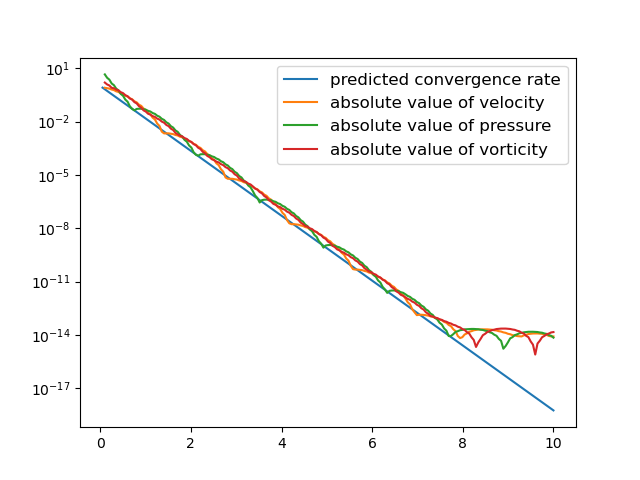
\includegraphics[width=\textwidth]{pic/rtp_cv.png}
    \caption{Numerical Convergence rate of return to Poiseuille flow in a straight channel}
    \label{fig:rtp_cv}
  \end{subfigure}
  \begin{subfigure}[b]{0.4\textwidth}
    \centering
    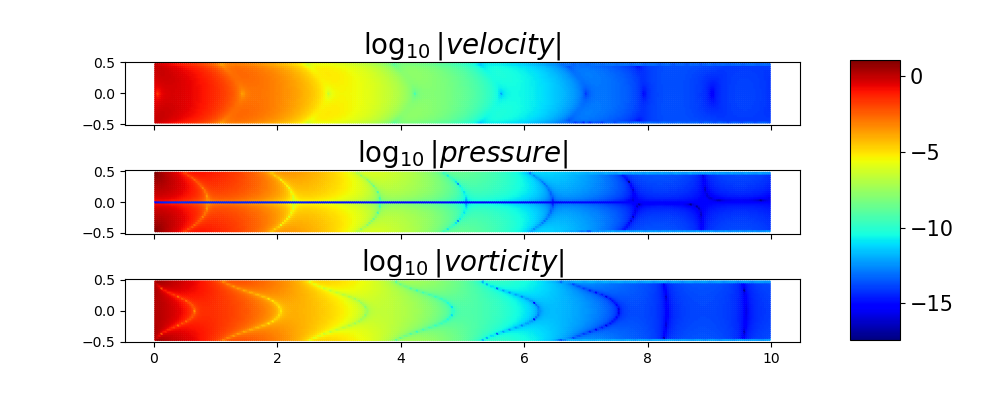
\includegraphics[width=\textwidth]{pic/rtppipe.png}
    \caption{$\log_{10}$ of the absolute value of the velocity, vorticity, and pressure within the straight channel.}
    \label{fig:rtppipe}
  \end{subfigure}
  \caption{Numerical exponential rate for return to Poiseuille flow. 
  This is solution of Stokes BVP on a straight channel of length 10 and width 1, 
  with non-slippery boundary condition on the top and bottom walls, 
  an incoming flow (smooth and randomly generated) of zero-net-flux on the left inlet, 
  and no outgoing flow on the right outlet. 
  (a) The semilogy of magnitude of velocity, pressure, and vorticity 
  along each vertical cross section along the channel. 
  % This agrees with the predicted converge rate in Section \ref{sec:ret2poi} all the way to 14th digits of accuracy. 
  (b) The color plot of the magnitude of velocity, pressure, and vorticity in $\log_{10}$ scale in the straight channel. 
  }
  \label{fig:r2pnumerical}
\end{figure}





\subsection{Numerical evidence of return to poiseuille}


The numerical evidence for return to Poiseuille phenomenon is 
demonstrated on a straight pipe of width $1$ and length $8$ as in Figure \ref{fig:r2pnumerical}. 
On the left boundary, a smooth velocity profile is imposed. 
This velocity profile is an arbitrarily picked smooth function that satisfies 
the requirement of equation (\ref{eq:velocity-condition-at-inlet}). 
On the rest of the curve, non-slippery condition is imposed.

Figure \ref{fig:rtp_cv} shows that the rate of returning 
to the zero flow is agreed with the 
predicted rate from Section \ref{sec:ret2poi} up to 14th digits of accuracy. 
Figure \ref{fig:rtppipe} is a color
plot where the color indicates the $\log_{10}$ of absolute value of the velocity, 
pressure, and vorticity. 




\subsection{a complicated network of pipes to show the power of this method}



\section{Conclusions\label{sec:conclusions}}


\section{Acknowledgements\label{sec:acknowledgements}}

We thank Charles S. Peskin and Manas Rachh for many useful discussions pretaining to this work.
We thank Manas Rachh and Libin Lu for providing support for the Flatiron Institute's FMM2D library \cite{FlatironinstituteFmm2d2022}.



\subsection{summarize what I've done}
\subsection{outlook. What other work might be followed?}
\bibliographystyle{plain}
\bibliography{references}


\end{document}
